\section{Positron Emission Tomography}
\label{sec.pet}


\begin{figure}[!b]
	\centering
	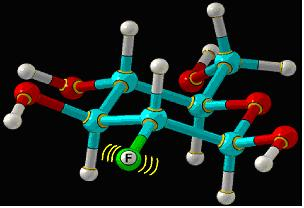
\includegraphics[scale=0.8]{img/MAPD_radiotracer.jpg}
	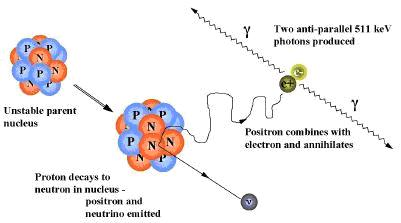
\includegraphics[scale=0.8]{img/MAPD_positronelectronannihilation.jpg}
	\caption{\label{fig.fdg}: Left panel, FDG is an organic molecule which contains a radioactive isotope of Fluor. The radionuclide decays emitting positrons, which annihilate after a short path length in the body tissue with an electron, resulting in the emission of two back-to-back photons of 511 keV (right panel). }
\end{figure}

A Positron Emission Tomography is a functional scan---it does not show anatomic features, but rather it measures metabolic activity of the cells of body tissues---. Used mostly in patients with brain or heart conditions and cancer, its big advantage is to identify the onset of a disease process before anatomical changes (that can be seen with other imaging processes such as computed tomography (CT) or MRI) related to the disease take place.

The PET technology  is based in the use of positron emitters radio-pharmaceuticals. 
If the biologically active molecule chosen is fluorodeoxyglucose (FDG), an analogue of glucose which contains a radioactive isotope of Fluor (F-18), the concentrations of tracer imaged will indicate tissue metabolic activity as it corresponds to the regional glucose uptake. Use of this tracer to explore the possibility of cancer metastasis (i.e., spreading to other sites) is the most common type of PET scan. However, many other radioactive tracers are used in PET to image the tissue concentration of other types of molecules of interest. 

Radioactive isotopes are produced (normally in a dedicated cyclotron) and attached to organic molecules that the studied cells absorb in their metabolism. The molecule and the radionuclide form the so called radiotracer. The tracer is injected to the patient where it will decay emitting a positron. The emitted positron travels a short distance before annihilating with an electron resulting in the emission of two 511 keV gamma rays in opposite directions (Figure \ref{fig.fdg}).

By detecting the two photons in coincidence and the coordinates of their interaction points in a rings of detectors surrounding the area under study is possible to define a line of response (LOR) along which the positron emitting source is located in the patient. A set of such intersecting lines allows 3D reconstruction of the source. The principle is illustrated in Figure \ref{fig.pet}.

\begin{figure}[!bthp]
	\centering
	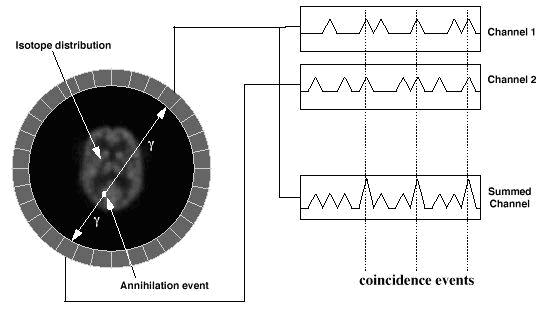
\includegraphics[scale=1.0]{img/MAPD_coincidenceprinciple.jpg}
	\caption{\label{fig.pet} Coincidence detection principle in a PET detector.}
\end{figure}

\subsection{Medical applications of PET}

\begin{figure}[!bthp]
	\centering
	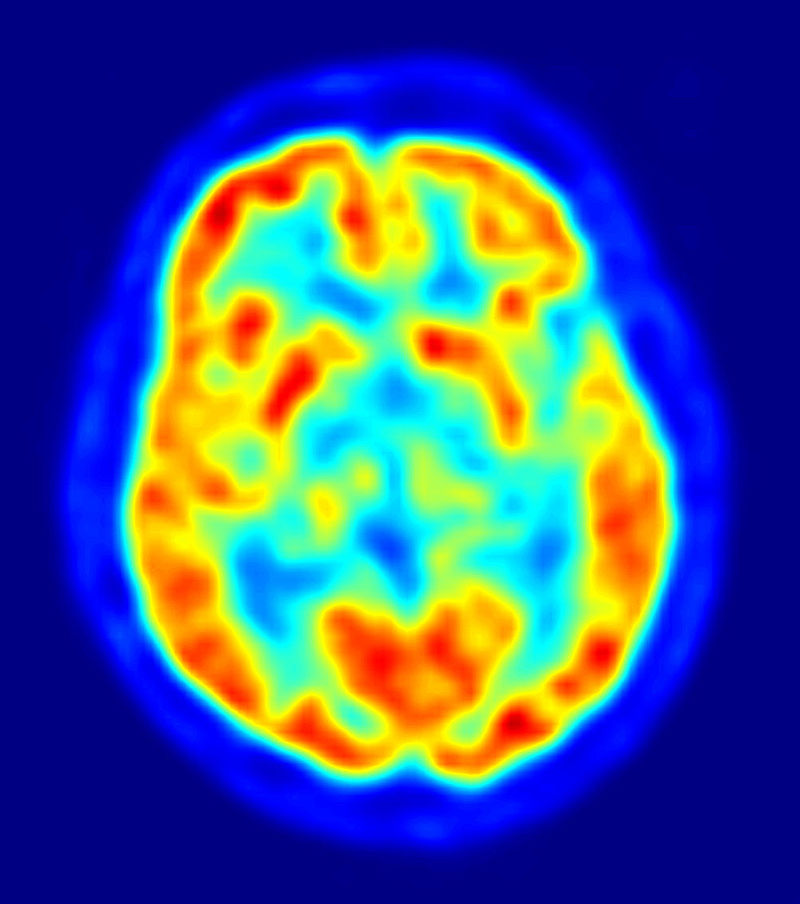
\includegraphics[scale=2.0]{img/800px-PET-image.jpg}
	\caption{\label{fig.brain} The image shows a transaxial slice of the brain of a 56 year old patient (male) taken with positron emission tomography (PET). The injected dose have been 282 MBq of FDG and the image was generated from a 20 minutes measurement with a ECAT Exact HR+ PET Scanner. Red areas show more accumulated tracer substance (FDG) and blue areas are regions where low to no tracer have been accumulated.}
\end{figure}

The main applications of PET to medicine are oncology, neuroimaging and cardiology. The oncological applications are mostly based in the use of FDG, a glucose analog where an atom of fluorine-18 (F-18) replaces an atom of oxygen. A typical dose of FDG used in an oncological scan has an effective radiation dose of 14 mSv, equivalent to about 5 years of dose by background radiation (combining natural and artificial sources). It follows that one of the important issues in PET applications is to reduce the FDG dose as much as possible, which in turn requires to improve the performance of the PET scanners.

FDG is taken up by glucose-using cells and phosphorylated\footnote{Phosphorylation is the addition of a phosphate (PO$_4^{3--}$) group to a protein or other organic molecule. Phosphorylation and its counterpart, dephosphorylation, turn many protein enzymes on and off, thereby altering their function and activity.} by hexokinase\footnote{An enzyme that phosphorylates hexoses (six-carbon sugars), forming hexose phosphate. In most organisms, glucose is the most important substrate of hexokinases, and glucose-6-phosphate the most important product.}. Because the oxygen atom that is replaced by F-18 to generate FDG is required for the next step in glucose metabolism in all cells, no further reactions occur in FDG. Furthermore, most tissues cannot remove the phosphate added by hexokinase. This means that FDG is trapped in any cell that takes it up, until it decays. This results in intense radiolabeling of tissues with high glucose uptake, such as the brain, the liver, and most cancers. As a result, FDG-PET can be used for diagnosis, staging, and monitoring treatment of many types of cancer. The technology is also very well suited to search for tumor metastasis, or for recurrence after a known highly active primary tumor is removed. 

PET neuroimaging uses the fact that the brain is an avid user of glucose, and since brain pathologies such as Alzheimer's disease greatly decrease brain metabolism of glucose standard FDG-PET of the brain, which measures regional glucose use, may also be successfully used to differentiate Alzheimer's disease from other dementing processes, and also to make early diagnosis of Alzheimer's disease. 

In clinical cardiology, FDG-PET can identify so-called ``hibernating myocardium'', that is a state when some segments of the myocardium exhibit abnormalities of contractile function. These abnormalities can also be visualized with echocardiography, cardiac magnetic resonance imaging or ventriculography. FDG-PET imaging of atherosclerosis to detect patients at risk of stroke is also feasible and can help test the efficacy of novel anti-atherosclerosis therapies.

One of the main limitations of the technology is the fact that  individual PET scans are more expensive than ``conventional'' imaging with computed tomography (CT) and magnetic resonance imaging (MRI). Reducing costs of PET scanners is, therefore, a major priority to facilitate the expansion of the technology. Conversely, the combination of PET with CT and MRI often leads to much improved scans, since the structural information offered by CT and MRI can be combined with the functional information offered by PET. 

In conclusion, the medical applications of PET can be improved by:
\begin{enumerate}
\item {\bf Increasing the performance of the PET scanner}, which in turn means improving the energy resolution, spatial resolution, coincidence resolution time and sensitivity, as will be discussed further beyond.
\item {\bf Reducing the cost of the PET scanner}, which requires the use of detection media which are cheaper than current solid scintillating detectors such as LSO/LYSO without compromising performance.
\item {\bf Combining PET with structural scans}, which, in the case of MRI requires the use of materials and sensors which can operate in the presence of very intense, highly variable magnetic fields. 
\end{enumerate}
